\documentclass[12pt]{article}%
%%%%%%%%%%%%%%%%%%%%%%%%%%%%%%%%%%%%%%%%%%%%%%%%%%%%%%%%%%%%%%%%%   
% All style files are available from 
%   http://wwww.uiuc.edu/~sariel/research/latex/
%%%%%%%%%%%%%%%%%%%%%%%%%%%%%%%%%%%%%%%%%%%%%%%%%%%%%%%%%%%%%%%%%%   


%%%%%%%%%%%%%%%%%%%%%%%%%%%%%%%%%%%%%%%%%%%%%%%%%%%%%%%%%%%%%%%%%%   
% Conditional compilation depending on whether this is my computer or
% not.
\IfFileExists{sariel_computer.sty}{\def\sarielComp{1}}{}
\ifx\sarielComp\undefined%
\newcommand{\SarielComp}[1]{}
\newcommand{\NotSarielComp}[1]{#1}%
\else
\newcommand{\SarielComp}[1]{#1}%
\newcommand{\NotSarielComp}[1]{}%
\fi
\newcommand{\IfPrinterVer}[2]{#2}%

%%%%%%%%%%%%%%%%%%%%%%%%%%%%%%%%%%%%%%%%%%%%%%%%%%%%%%%%%%%%%%%%%% 


\usepackage[cm]{fullpage}%
\usepackage{amsmath}%
\usepackage{amssymb}%
\usepackage[cmyk]{xcolor}%
%\usepackage{xcolor}%

\SarielComp{\usepackage{sariel_colors}}%

\usepackage[amsmath,thmmarks]{ntheorem}%
\theoremseparator{.}%

\usepackage{titlesec}%
\titlelabel{\thetitle. }%

\usepackage{graphicx}%
\usepackage{xcolor}%
\usepackage{mleftright}%
\usepackage{xspace}%
\usepackage{hyperref}%

\usepackage{caption}%

\newcommand{\hrefb}[3][black]{\href{#2}{\color{#1}{#3}}}%

\IfPrinterVer{%
   \usepackage{hyperref}%
}{%
   \usepackage{hyperref}%
   \hypersetup{%
      breaklinks,%
      ocgcolorlinks, colorlinks=true,%
      urlcolor=[rgb]{0.25,0.0,0.0},%
      linkcolor=[rgb]{0.5,0.0,0.0},%
      citecolor=[rgb]{0,0.2,0.445},%
      filecolor=[rgb]{0,0,0.4},
      anchorcolor=[rgb]={0.0,0.1,0.2}%
   }
   % \usepackage{cleveref}
}

% ----------------------------------------------------------------------
% ----------------------------------------------------------------------
% Defining theorem like environments
% ----------------------------------------------------------------------
% ----------------------------------------------------------------------
\theoremseparator{.}%

\theoremstyle{plain}%
\newtheorem{theorem}{Theorem}[section]

\newtheorem{lemma}[theorem]{Lemma}
\newtheorem{conjecture}[theorem]{Conjecture}
\newtheorem{corollary}[theorem]{Corollary}
\newtheorem{claim}[theorem]{Claim}%
\newtheorem{fact}[theorem]{Fact}
\newtheorem{observation}[theorem]{Observation}
\newtheorem{invariant}[theorem]{Invariant}
\newtheorem{question}[theorem]{Question}
\newtheorem{proposition}[theorem]{Proposition}
\newtheorem{prop}[theorem]{Proposition}
\newtheorem{openproblem}[theorem]{Open Problem}

\theoremstyle{plain}%
\theoremheaderfont{\sf} \theorembodyfont{\upshape}%
\newtheorem*{remark:unnumbered}[theorem]{Remark}%
\newtheorem*{remarks}[theorem]{Remarks}%
\newtheorem{remark}[theorem]{Remark}%
\newtheorem{definition}[theorem]{Definition}
\newtheorem{defn}[theorem]{Definition}
\newtheorem{example}[theorem]{Example}
\newtheorem{exercise}[theorem]{Exercise}
\newtheorem{problem}[theorem]{Problem}
\newtheorem{xca}[theorem]{Exercise}
\newtheorem{exercise_h}[theorem]{Exercise}
\newtheorem{assumption}[theorem]{Assumption}%

% Proof environment
\newcommand{\myqedsymbol}{\rule{2mm}{2mm}}

\theoremheaderfont{\em}%
\theorembodyfont{\upshape}%
\theoremstyle{nonumberplain}%
\theoremseparator{}%
\theoremsymbol{\myqedsymbol}%
\newtheorem{proof}{Proof:}%

\newtheorem{proofof}{Proof of\!}%

% theorem block end
%%%%%%%%%%%%%%%%%%%%%%%%%%%%%%%%%%%%%%%%%%%%%%%%%%%%%%%%%%%%%%%%%%%%


%%%%%%%%%%%%%%%%%%%%%%%%%%%%%%%%%%%%%%%%%%%%%%%%%%%%%%%%%%%%%%%%%% 5
% Color emph
\providecommand{\emphind}[1]{\emph{#1}\index{#1}}
\definecolor{nalmostblack}{rgb}{0, 0, 0.7}
\providecommand{\emphic}[2]{%
   \textcolor{nalmostblack}{%
      \textbf{\emph{#1}}}%
   \index{#2}}


\providecommand{\emphi}[1]{\emphic{#1}{#1}}

\definecolor{almostblack}{rgb}{0, 0, 0.5}
\providecommand{\emphw}[1]{{\emph{{\textcolor{almostblack}{#1}}}}}%

\providecommand{\emphOnly}[1]{\emph{\textcolor{almostblack}{\textbf{#1}}}}
% Color emph - end 
%%%%%%%%%%%%%%%%%%%%%%%%%%%%%%%%%%%%%%%%%%%%%%%%%%%%%%%%%%%%%%%%%% 5


\numberwithin{figure}{section}%
\numberwithin{table}{section}%
\numberwithin{equation}{section}%


%%%%%%%%%%%%%%%%%%%%%%%%%%%%%%%%%%%%%%%%%%%%%%%%%%%%%%%%%%%%%%%%%%%
% Sariel's thanks
%%%%%%%%%%%%%%%%%%%%%%%%%%%%%%%%%%%%%%%%%%%%%%%%%%%%%%%%%%%%%%%%%%% 

\providecommand{\tildegen}{{\protect\raisebox{-0.1cm}
      {\symbol{'176}\hspace{-0.01cm}}}}
\newcommand{\atgen}{\symbol{'100}}
\newcommand{\SarielThanks}[1]{\thanks{Department of Computer Science;
      University of Illinois; 201 N. Goodwin Avenue; Urbana, IL,
      61801, USA; {\tt sariel\atgen{}illinois.edu}; {\tt
         \url{http://sarielhp.org/}.} #1}}


%%%%%%%%%%%%%%%%%%%%%%%%%%%%%%%%%%%%%%%%%%%%%%%%%%%%%%%%%%%%%%%%%%%%%%
%    Handling references
%%%%%%%%%%%%%%%%%%%%%%%%%%%%%%%%%%%%%%%%%%%%%%%%%%%%%%%%%%%%%%%%%%%%%%

\newcommand{\HLink}[2]{\hyperref[#2]{#1~\ref*{#2}}}
\newcommand{\HLinkSuffix}[3]{\hyperref[#2]{#1\ref*{#2}{#3}}}

\newcommand{\figlab}[1]{\label{fig:#1}}
\newcommand{\figref}[1]{\HLink{Figure}{fig:#1}}

\newcommand{\thmlab}[1]{{\label{theo:#1}}}
\newcommand{\thmref}[1]{\HLink{Theorem}{theo:#1}}

\newcommand{\corlab}[1]{\label{cor:#1}}
\newcommand{\corref}[1]{\HLink{Corollary}{cor:#1}}%

\providecommand{\deflab}[1]{\label{def:#1}}
\newcommand{\defref}[1]{\HLink{Definition}{def:#1}}


\newcommand{\clmlab}[1]{\label{claim:#1}}
\newcommand{\clmref}[1]{\HLink{Claim}{claim:#1}}

\newcommand{\apndlab}[1]{\label{apnd:#1}}
\newcommand{\apndref}[1]{\HLink{Appendix}{apnd:#1}}

\newcommand{\seclab}[1]{\label{sec:#1}}
\newcommand{\secref}[1]{\HLink{Section}{sec:#1}}
\newcommand{\rectA}{\Mh{B}}%
\newcommand{\rectB}{\Mh{D}}%
\newcommand{\clientsY}[2]{\Mh{\mathsf{C}}\pth{#1,#2}}

\newcommand{\DW}{\times}
\newcommand{\ConeSet}{\Mh{\mathcal{C}}}%
\newcommand{\shrinkDY}[2]{#1_{\boxminus #2}}
\newcommand{\Rects}{\Mh{\mathcal{R}}}%


\newcommand{\itemlab}[1]{\label{item:#1}}
\newcommand{\itemref}[1]{\HLinkSuffix{}{item:#1}{}}

\newcommand{\lemlab}[1]{\label{lemma:#1}}
\newcommand{\lemref}[1]{\HLink{Lemma}{lemma:#1}}%

\providecommand{\eqlab}[1]{}%
\renewcommand{\eqlab}[1]{\label{equation:#1}}
\newcommand{\Eqref}[1]{\HLinkSuffix{Eq.~(}{equation:#1}{)}}

%%%%%%%%%%%%%%%%%%%%%%%%%%%%%%%%%%%%%%%%%%%%%%%%%%%%%%%%%%%%%%%%%%% 
% Sariel's standard commands...
%%%%%%%%%%%%%%%%%%%%%%%%%%%%%%%%%%%%%%%%%%%%%%%%%%%%%%%%%%%%%%%%%%% 

\newcommand{\remove}[1]{}%
\newcommand{\Set}[2]{\left\{ #1 \;\middle\vert\; #2 \right\}}
\newcommand{\pth}[2][\!]{\mleft({#2}\mright)}%
\newcommand{\pbrcx}[1]{\left[ {#1} \right]}%
\newcommand{\Prob}[1]{\mathop{\mathbf{Pr}}\!\pbrcx{#1}}
\newcommand{\Ex}[2][\!]{\mathop{\mathbf{E}}#1\pbrcx{#2}}

\newcommand{\ceil}[1]{\left\lceil {#1} \right\rceil}
\newcommand{\floor}[1]{\left\lfloor {#1} \right\rfloor}

\newcommand{\brc}[1]{\left\{ {#1} \right\}}
\newcommand{\cardin}[1]{\left| {#1} \right|}%

\renewcommand{\th}{th\xspace}
\newcommand{\ds}{\displaystyle}%

\renewcommand{\Re}{\mathbb{R}}%
\newcommand{\reals}{\Re}%


%%%%%%%%%%%%%%%%%%%%%%%%%%%%%%%%%%%%%%%%%%%%%%%%%%%%%%%%%%%%%%%%%%%%%%%%%
% Defining comptenum environment using enumitem
\usepackage[inline]{enumitem}

\newlist{compactenumA}{enumerate}{5}%
\setlist[compactenumA]{topsep=0pt,itemsep=-1ex,partopsep=1ex,parsep=1ex,%
   label=(\Alph*)}%

\newlist{compactenuma}{enumerate}{5}%
\setlist[compactenuma]{topsep=0pt,itemsep=-1ex,partopsep=1ex,parsep=1ex,%
   label=(\alph*)}%

\newlist{compactenumI}{enumerate}{5}%
\setlist[compactenumI]{topsep=0pt,itemsep=-1ex,partopsep=1ex,parsep=1ex,%
   label=(\Roman*)}%

\newlist{compactenumi}{enumerate}{5}%
\setlist[compactenumi]{topsep=0pt,itemsep=-1ex,partopsep=1ex,parsep=1ex,%
   label=(\roman*)}%

\newlist{compactitem}{itemize}{5}%
\setlist[compactitem]{label=\ensuremath{\bullet}}%
\setlist[compactitem]{topsep=0pt,itemsep=-1ex,partopsep=1ex,parsep=1ex,%
   label=\ensuremath{\bullet}}%


\usepackage{stmaryrd}%
\providecommand{\IntRange}[1]{\mleft\llbracket #1 \mright\rrbracket}
\newcommand{\IRX}[1]{\IntRange{#1}}%
\newcommand{\IRY}[2]{\left\llbracket #1:#2 \right\rrbracket}

%%%%%%%%%%%%%%%%%%%%%%%%%%%%%%%%%%%%%%%%%%%%%%%%%%%%%%%%%%%%%%%%%%%%%%%%%%

\usepackage{wasysym}

\newcommand{\disk}{\Mh{\ocircle}}
\newcommand{\diskVY}[2]{\disk_{\downarrow}^{#1}\pth{#2}}%




%%%%%%%%%%%%%%%%%%%%%%%%%%%%%%%%%%%%%%%%%%%%%%%%%%%%%%%%%%%%%%%%%%% 
%%%%%%%%%%%%%%%%%%%%%%%%%%%%%%%%%%%%%%%%%%%%%%%%%%%%%%%%%%%%%%%%%%% 
% Papers specific commands...
%%%%%%%%%%%%%%%%%%%%%%%%%%%%%%%%%%%%%%%%%%%%%%%%%%%%%%%%
%%%%%%%%%%%%%%%%%%%%%%%%%%%%%%%%%%%%%%%%%%%%%%%%%%%%%%%%

\providecommand{\Mh}[1]{#1}%

\newcommand{\eps}{\varepsilon}

\newcommand{\CC}{\Mh{\mathcal{C}}}%
\newcommand{\FF}{\Mh{\mathcal{F}}}%
\newcommand{\LL}{\mathcal{L}}
\newcommand{\DT}{\Mh{\mathcal{D}}}%
\newcommand{\DTX}[1]{\Mh{\mathcal{DT}}\pth{#1}}
\newcommand{\DG}{\mathcal{DG}}

\newcommand{\etal}{\textit{et~al.}\xspace}

\newcommand{\Term}[1]{\textsf{#1}}
\newcommand{\TermI}[1]{\Term{#1}\index{#1@\Term{#1}}}

\newcommand{\QSPD}{\Term{QSPD}\xspace}

\newcommand{\StavThanks}[1]{%
   \thanks{Department of Computer Science;
      University of Illinois; 201 N. Goodwin Avenue; Urbana, IL,
      61801, USA; {\tt stava2\atgen{}illinois.edu}; {\tt
         \url{https://publish.illinois.edu/stav-ashur}.} #1}}

\newcommand{\pa}{\Mh{p}}%
\newcommand{\pb}{\Mh{q}}%
\newcommand{\pc}{\Mh{u}}%
\newcommand{\pd}{\Mh{v}}%

\newcommand{\px}{\Mh{x}}%
\newcommand{\py}{\Mh{y}}%
\newcommand{\pz}{\Mh{z}}%

\newcommand{\dGY}[2]{\Mh{\mathsf{d}}\pth{#1,#2}}%
\newcommand{\dGZ}[3]{\Mh{\mathsf{d}_{#1}}\pth{#2,#3}}%
\newcommand{\dY}[2]{\left\| #1 - #2 \right\|}%


\newcommand{\dsZ}[3]{\Mh{\mathsf{d}}_{#1}\pth{#2, #3}}%
\newcommand{\dZ}[3]{\left\| #2 - #3 \right\|_{#1}}%

\newcommand{\dsY}[2]{\mathsf{d}\pth{#1,#2}}
\newcommand{\DistSetY}[2]{\dsY{#1}{#2}}%

\newcommand{\body}{\Mh{C}}%

\newcommand{\grid}{\Mh{\mathsf{K}}}%

\providecommand{\G}{\Mh{G}}%
\renewcommand{\G}{\Mh{G}}%

\newcommand{\GA}{\Mh{H}}%

\providecommand{\GB}{\Mh{I}}%
\renewcommand{\GB}{\Mh{I}}%


\newcommand{\PS}{\Mh{P}}%
\newcommand{\PSup}{\Mh{P}_\uparrow}%
\newcommand{\PSdown}{\Mh{P}_\downarrow}%

\newcommand{\QS}{\Mh{\mathcal{Q}}}%
\newcommand{\liftX}[1]{\mathrm{lift}\pth{#1}}%

\newcommand{\rect}{\Mh{R}}%

\newcommand{\EG}{\Mh{E}}%
\newcommand{\EGX}[1]{\Mh{E}\pth{#1}}%
\newcommand{\region}{\Mh{\mathcalb{r}}}%
\newcommand{\gminus}{-}%
\newcommand{\interiorX}[1]{\mathrm{int}\pth{#1}}%
\newcommand{\restrictY}[2]{#1 \cap {#2}}

\newcommand{\cpX}[1]{\Mh{\mathrm{c{}p}}\pth{#1}}%
\newcommand{\diamX}[1]{\mathrm{diam}\pth{#1}}%

\newcommand{\spread}{\Mh{\Phi}}
\newcommand{\spreadX}[1]{\spread\pth{#1}}

\newcommand{\WS}{\Mh{\mathcal{W}}}%
\newcommand{\WeightX}[1]{\Mh{\omega} \pth{#1}}
\newcommand{\diameterX}[1]{\mathrm{d{}i{}am}\pth{#1}}

\newcommand{\SSPD}{\Term{SSPD}\xspace}%

\newcommand{\PSB}{\Mh{B}}%
\newcommand{\PSC}{\Mh{C}}%

\newcommand{\PSX}{\Mh{X}}%
\newcommand{\PSY}{\Mh{Y}}%

\newcommand{\WSPD}{\Term{WSPD}\xspace}%

\newcommand{\coneY}[2]{\mathrm{cone}\pth{#1,#2}}%
\newcommand{\IS}{\Mh{\mathcal{I}}}%
\newcommand{\epsA}{\Mh{\vartheta}}%

\newcommand{\GY}[2]{\Mh{\mathcal{G}}\pth{#1, #2}}%
\newcommand{\cen}{\Mh{c}}%
\newcommand{\Pair}{\Mh{\Xi}}%

\newcommand{\XSays}[2]{{ {$\rule[-0.12cm]{0.2in}{0.5cm}$\fbox{\tt #1:}
      } #2 \marginpar{\textcolor{red}{#1}}
      {$\rule[0.1cm]{0.3in}{0.1cm}$\fbox{\tt
            end}$\rule[0.1cm]{0.3in}{0.1cm}$} } }
\newcommand{\sariel}[1]{{\XSays{Sariel}{#1}}}
\newcommand{\Sariel}[1]{{\XSays{Sariel}{#1}}}

\newcommand{\QSup}{\QS_{\uparrow}}
\newcommand{\QSdown}{\QS_{\downarrow}}


%%%%%%%%%%%%%%%%%%%%%%%%%%%%%%%%%%%%%%%%%%%%%%%%%%%%%%%%%%%%%%%%%%
%%%%%%%%%%%%%%%%%%%%%%%%%%%%%%%%%%%%%%%%%%%%%%%%%%%%%%%%%%%%%%%%%%
%%%%%%%%%%%%%%%%%%%%%%%%%%%%%%%%%%%%%%%%%%%%%%%%%%%%%%%%%%%%%%%%%%
% Restating lemmas/theorems...
%
% Example
%---------------------------------------------------------------------
% \SaveContent{\LemmaNumVerticesDepthBody}{ BLA BLA }
% 
% \begin{lemma}[{{\normalfont Proof in \apndref{num:v:depth}}}]
%       \lemlab{num:vertices:depth}%
%       \LemmaNumVerticesDepthBody{}
% \end{lemma}
%...
% \bigskip%
% \RestatementOf{\lemref{num:vertices:depth}}{\LemmaNumVerticesDepthBody}
%---------------------------------------------------------------------

\newcommand{\SaveContent}[2]{%
   \expandafter\newcommand{#1}{#2}%
}

\newcommand{\RestatementOf}[2]{
   \noindent%
   \textbf{Restatement of #1.}
   % 
   {\em #2{}}%
}

%%% End
%%%%%%%%%%%%%%%%%%%%%%%%%%%%%%%%%%%%%%%%%%%%%%%%%%%%%%%%%%%%%%%%%%
%%%%%%%%%%%%%%%%%%%%%%%%%%%%%%%%%%%%%%%%%%%%%%%%%%%%%%%%%%%%%%%%%%


%%%%%%%%%%%%%%%%%%%%%%%%%%%%%%%%%%%%%%%%%%%%%%%%%%%%%%%%%%%%%%%%%%%%%%%%
%%%%%%%%%%%%%%%%%%%%%%%%%%%%%%%%%%%%%%%%%%%%%%%%%%%%%%%%%%%%%%%%%%%%%%%%
% \mathcalb - a different font that looks a bit like mathcal

\DeclareFontFamily{U}{BOONDOX-calo}{\skewchar\font=45 }
\DeclareFontShape{U}{BOONDOX-calo}{m}{n}{<-> s*[1.05] BOONDOX-r-calo}{}
\DeclareFontShape{U}{BOONDOX-calo}{b}{n}{<-> s*[1.05] BOONDOX-b-calo}{}
\DeclareMathAlphabet{\mathcalb}{U}{BOONDOX-calo}{m}{n}
\SetMathAlphabet{\mathcalb}{bold}{U}{BOONDOX-calo}{b}{n}
\DeclareMathAlphabet{\mathbcalb}{U}{BOONDOX-calo}{b}{n}

% \mathcalb - end of file
%%%%%%%%%%%%%%%%%%%%%%%%%%%%%%%%%%%%%%%%%%%%%%%%%%%%%%%%%%%%%%%%
%%%%%%%%%%%%%%%%%%%%%%%%%%%%%%%%%%%%%%%%%%%%%%%%%%%%%%%%%%%%%%%%

\newcommand{\CHX}[1]{\mathsf{ch}\pth{#1}}%

\newcommand{\rinX}[1]{\Mh{r}_{\mathrm{in}}\pth{#1}}%
\newcommand{\routX}[1]{\Mh{R}_{\mathrm{out}}\pth{#1}}%
\newcommand{\arX}[1]{\Mh{\mathsf{a{}r}}\pth{#1}}%
\newcommand{\Elp}{\Mh{\mathcal{E}}}

\newcommand{\cell}{\Mh{\mathsf{C}}}%

\newcommand{\Of}{\Mh{\mathcal{O}}}%
\newcommand{\Oeps}{\Mh{\mathcal{O}_\eps}}%
\newcommand{\gConst}{\Mh{\tau}}%
\newcommand{\xSlabX}[1]{\overleftrightarrow{#1}}
\newcommand{\ySlabX}[1]{\updownarrow\!{#1}}
\newcommand{\widthX}[1]{\Mh{\mathsf{wd}}\pth{#1}} \smallskip%

\newcommand{\HERE}{%
   {\noindent\hspace{-1cm}\rule{1.2\linewidth}{4cm}}   
   % \rule{4cm}{4cm}
}

%%%%%%%%%%%%%%%%%%%%%%%%%%%%%%%%%%%%%%%%%%%%%%%%%%%%%%%%
%%BeginIpePreamble
%%%%%%%%%%%%%%%%%%%%%%%%%%%%%%%%%%%%%%%%%%%%%%%%%%%%%%%%

\newcommand{\sqr}{\mathcalb{s}}%
\newcommand{\sqrA}{\mathcalb{t}}%
\newcommand{\sqrB}{\mathcalb{u}}%

\newcommand{\polylog}{\mathop{\mathrm{polylog}}}%

%%%%%%%%%%%%%%%%%%%%%%%%%%%%%%%%%%%%%%%%%%%%%%%%%%%%%%%%
%%EndIpePreamble
%%%%%%%%%%%%%%%%%%%%%%%%%%%%%%%%%%%%%%%%%%%%%%%%%%%%%%%%



%



\begin{document}

\title{Fault-Tolerant and Local Spanners Revisited}
	
\author{%
   Stav Ashur%
   \StavThanks{}%
   \and%
   Sariel Har-Peled%
   \SarielThanks{Work on this paper was partially supported by a
      NSF AF award CCF-1907400.  }%
}%
	
\maketitle


\section{Introduction}

\paragraph{Euclidean graph and spanners.}
For a set $\PS$ of points in $\Re^d$, an \emphw{Euclidean graph}
$\G = (\PS, \EG)$ is an undirected graph with $\PS$ as the set of
vertices. An edge $\pa \pb \in \EG$ is naturally associated with the
segment $\pa\pb$, and weight of the edge is the (Euclidean) length of
the segment.  Consider a pair of points $\pa,\pb \in \PS$. For a
parameter $t \geq 1$, a path between $\pa$ and $\pb$ in $\G$ is a
\emphw{$t$-path} if the length of the path is at most
$t \dY{\pa}{\pb}$, where $\dY{\pa}{\pb}$ is the Euclidean distance
between $\pa$ and $\pb$.  The graph $\G$ is a \emphw{$t$-spanner} of
$\PS$ if there is a $t$-path between any pair of points
$\pa,\pb\in \PS$.  Throughout the paper, $n$ denotes the cardinality
of the point set $\PS$, unless stated otherwise. We denote the length
of the shortest path between $\pa,\pb\in \PS$ in the graph $\G$ by
$\dGY{\pa}{\pb}$.

\paragraph{Residual graphs.}

Let $\FF$ be a family of regions in the plane. For a fault region
$\region \in \FF$ and a geometric graph $\G$ on a point set $\PS$, let
$\G \gminus \region$ be the residual graph after removing from it all
the points of $\PS$ in $\region$. and all the edges that intersects
$\region$.  Formally, let
\begin{equation*}
    \G \gminus \region%
    =%
    \bigl( \PS \setminus \region, \Set{ uv \in \EG }{ uv \cap
       \interiorX{\region} = \emptyset} \bigr),
\end{equation*}
where $\interiorX{\region}$ denotes the interior of
$\region$. Similarly, let
\begin{equation*}
    \restrictY{\G}{\region}%
    =%
    \bigl( \PS \cap \interiorX{\region},
    \Set{uv \in \EG}{ uv \subseteq \interiorX{\region} } \bigr).
\end{equation*}
be the residual graph after restricting $\G$ to the region $\region$.

\paragraph{Fault-tolerant and local spanners.}

A \emphw{fault-tolerant spanner} for $\FF$, is a graph $\G$, such that
for any region $\region$ (i.e., the ``attack''), the graph
$\G \gminus \region$ is a $t$-spanner for all its
vertices. Surprisingly, as shown by Abam \etal \cite{abfg-rftgs-09},
such fault-tolerant spanners can be constructed where the attack
region is any convex set. Furthermore, these spanners have near linear
number of edges.

In the same spirit, a graph $\G$ is a \emphw{local spanner} for $\FF$,
if for any region $\region \in \FF$, we have that
$\restrictY{\G}{\region}$ is a $t$-spanner for all its vertices.  The
notion of local-spanner was defined by Abam and Borouny
\cite{ab-lgs-21}. They showed how to construct such spanners for
axis-parallel squares and vertical slabs. They also showed how to
construct such spanners for disks, if one is allowed to add Steiner
points. Abam and Borouny left the question of how to construct local
spanners for disks as an open problem.

\subsection*{Our results}

We present a new construction of spanners, which surprisingly, is not
only fault-tolerant for convex regions, but it also a local spanner
for disks. This resolves the aforementioned open problem from Abam and
Borouny \cite{ab-lgs-21}. Our construction is a variant of the
original construction of Abam \etal \cite{abfg-rftgs-09}.

We then investigate various other constructions of local spanners,
where one is allowed to slightly shrink the region.
	

%%%%%%%%%%%%%%%%%%%%%%%%%%%%%%%%%%%%%%%%%%%%%%%%%%%%%%%%%%%%%%%%%%%%%%%%%
%%%%%%%%%%%%%%%%%%%%%%%%%%%%%%%%%%%%%%%%%%%%%%%%%%%%%%%%%%%%%%%%%%%%%%%%%
%%%%%%%%%%%%%%%%%%%%%%%%%%%%%%%%%%%%%%%%%%%%%%%%%%%%%%%%%%%%%%%%%%%%%%%%%

\section{Complement of disk faults / disk local spanners}
	
%%%%%%%%%%%%%%%%%%%%%%%%%%%%%%%%%%%%%%%%%%%%%%%%%%%%%%%%%%%%%%%%%%%%%%%%%
%%%%%%%%%%%%%%%%%%%%%%%%%%%%%%%%%%%%%%%%%%%%%%%%%%%%%%%%%%%%%%%%%%%%%%%%%
%%%%%%%%%%%%%%%%%%%%%%%%%%%%%%%%%%%%%%%%%%%%%%%%%%%%%%%%%%%%%%%%%%%%%%%%%
	
\section{Convex faults / disk local spanners}

=======
   \SarielThanks{Work on this paper was partially supported by a
      NSF AF award CCF-1907400.  }%
}%
	
\maketitle
	
\section{Introduction}
	
Let $\FF$ be a family of regions in the plane, which we call the fault
regions. For a fault region $F\in \FF$ and a geometric graph $G$ on a
point set $P$ , we define $G\ominus F$ to be the part of $G$ that
remains after the points of $P$ that are contained in $F$, and all the
edges of $G$ that intersect $F$ have been removed from the graph. For
simplicity, we assume that a region fault $F$ does not contain its
boundary, i.e., only vertices and edges intersecting the interior of
$F$ will be affected.
	
	
Let $\LL$ be a family of regions in the plane, which we call the local
regions. For a local region $L\in \LL$ and a geometric graph $G$ on a
point set $P$ , we define $G\mid_F$ to be the part of $G$ contained in
the interior of $F$, meaning only the vertices and edges that are
fully contained in the interior of $F$.
	
Formally, given $G=(P,E)$:
	
$$G\ominus F = (p\setminus F, \{e\in E~|~ e\cap F = \emptyset\})$$

$$G\mid_F = (p \cap F, \{e\in E~|~ e\subseteq F\})$$
	
\paragraph{The problems:}

\begin{enumerate}
    \item Given a set $P$ of points in $\Re^2$, and a family $\FF$ of
    regions, compute a graph $G$ such that $G\ominus F$ is a
    $t$-spanner of $P$ for any fault $F\in\FF$
    \item Given a set $P$ of points in $\Re^2$, and a family $\LL$ of
    regions, compute a graph $G$ such that $G\mid_F$ is a $t$-spanner
    for any local region $L\in\LL$
\end{enumerate}
.

	
\section{Complement of disk faults / disk local spanners}
	
	
\section{Convex faults / disk local spanners}
>>>>>>> 1eb5c890e1265a08cfd6d0936ebc605ac6255af5
Let $\FF$ be the set of convex regions, and $\eps>0$. We use the
construction of Abam \etal \cite{abfg-rftgs-09} in order to create a
$(1+\eps)$-$\FF$ tolerant spanner. In their paper, Abam \etal build a
\emph{semi separated pair decomposition} (SSPD), and add a set of
carefully chosen edges between every two sets $A,B\subseteq P$ that
compose a pair in the SSPD. Given a pair $(A,B)$, the algorithm
partitions the larger set, w.l.o.g it is $B$, by shooting rays at
fixed angular intervals from a disk that contains $A$, and then adds a
planar set of edges $E_i$ between the convex hulls of $A$ and every
part $B$ of $B$, that has the following property:

For any half-plane $H$ such that $A\cap H\neq \emptyset$ and
$B\cap H\neq \emptyset$, there exists an edge $e\in E_i$ such that
$e\subseteq H$. This property, together with the properties of the
SSPD, makes the resulted graph an $\FF$-fault tolerant spanner.

We notice, that a similar construction that chooses $E_i$ to be the
edges of the Delaunay triangulation with one end in $A$ and the other
in $B$ has the same property. We now prove that for any disk
$d\subseteq \Re^2$, and for any set $P'$ of points we have that
$\DT(P')\mid_d$ is connected. This is enough as half-planes can be
simulated by complements of disks.

\begin{claim}
    For a set of points $P\subseteq \Re^2$ and for any disk $d$,
    $\DT(P)\mid_d$ is connected.
\end{claim}

\begin{proof}
    We prove a different claim that immediately implies the desired
    one. Let $d$ be a disk with two points $p,q\in P$ on its
    boundary. Then there is a path between $p$ and $q$ in
    $\DT(P)\mid_d$. This is enough as for every two points $p,q$ and a
    disk $d$ containing them, we can get a disk $d'$ that contains $p$
    and $q$ on it's boundary by moving the center of $d$ in an
    arbitrary direction until either of them, say $p$ is on the
    boundary, and them moving the center of the disk towards $p$ while
    shrinking the size of the disk to maintain $p$ on the boundary,
    until $q$ as well is on the boundary.
    
    We prove by induction over the number points in the interior of
    $d$.
    
    $|d\cap (P\setminus \partial d)| = 0$: Then by construction of the Delaunay triangulation the edge $\{p,q\}$ is in $\DT(P)$ and is contained in the interior of $D$.\\
    
    $|d\cap (P\setminus \partial d)| > 0$: Let $x\in P$ be a point in
    the interior of $d$. We move the center of $d$ in the direction of
    $p$, shrinking $d$ in the process, until we get a disk
    $d'\subseteq d$ such that $x$ is on the boundary of $d'$. By
    induction there is a path between $p$ and $x$ in $\DT\mid_{d'}$,
    and since $\DT\mid_{d'}\subseteq \DT\mid_{d}$ we have that the
    same path exists in $\DT\mid_{d}$. The same proof gives us a path
    between $x$ and $q$ and thus we are done.
    
\end{proof}

Since the triangulation is planar, all of the arguments from the
original paper regarding the size of the spanner hold, and we get a
$(1+\eps)-\FF$ fault tolerant spanner of size $O(\eps^{-3}n\log n)$ in
$O(\eps^{-2}n\log n)$ time.

\section{Complement of convex faults / convex local spanners}
Using the same argument, we can extend the result for the case where
$\LL$ is the set of all scaled and translated copies, homothets, of a
convex shape $\CC$. While the Delaunay triangulation is not well
defined for all convex shapes, the operation of creating edges between
two points $p,q\in P$ such that there exist a homothet of $\CC$ that
<<<<<<< HEAD
contains only $p$ and $q$ and no other point of $\PS$ is always well
defined, and gives us a graph known as the $\CC$-Delaunay graph of
$\PS$, and denoted $\DG_{\CC}(P)$. The above proof applies almost
=======
contains only $p$ and $q$ and no other point of $P$ is always well
defined, and gives us a graph known as the $\CC$-Delaunay graph of
$P$, and denoted $\DG_{\CC}(P)$. The above proof applies almost
>>>>>>> 1eb5c890e1265a08cfd6d0936ebc605ac6255af5
verbatim for any convex $\CC$, and proves the connectivity of
$\DG_{\CC}(P)$ for any $L\in \LL$.

We need only to define a suitable shrinking operation for convex
region towards a point, which is possible, for example, by
parameterizing the curve defining the region and leaving the desired
point in the same coordinate of the smaller curve. So, we get a
$(1+\eps)-\LL$ local spanner of size $O(\eps^{-3}n\log n)$ in
$O(\eps^{-2}n\log n)$ time.(

%	TODO: this is actually not true unless we know how to build
% \DG_{\C}(P)

%	Since the Delaunay triangulation is well defined for the
% \emph{polygonal convex distance} (L.P. Chew and
<<<<<<< HEAD
% R.L. Drydale. Voronoi diagrams based on convex distance functions.In
% 1st SoCG, pages 234–244, ACM Press, 1985), we can use the exact same
% proof (again replacing only the distance function and the disk) to
% get an algorithm for this entire family of problems.

\section{$\eps$-shadow}

In this section we consider a weaker form of fault tolerance. Given a
family $\LL$ of shapes, we say that $\G$ is a $(\LL,\eps)$-local
spanner if for any $L\in\LL$ we have that $G\mid_{L_{\eps}}$, where
$L_{\eps}$ is $L$ rescaled by $(1-\eps)$, is a $t$-spanner. We call
$L\setminus L_{\eps}$ the \emph{shadow} of $L$, and we say that a
point $p$ is \emph{truly contained} in $L$ w.r.t. $\eps$, and denote
$p\in_{\eps} L$, if $p\in L_{\eps}$.

\subsection{Bounded aspect ratio rectangles}
Let $\LL$ be the set of axis parallel rectangles with aspect ratio at
most $1<\alpha$. We repeatedly preform the algorithm for convex local
spanners with rectangles of different aspect-ratio, where in the
$i$\th iteration we use a rectangle with aspect ratio
$\left(1+\eps\right)^i$, where $i\in\{0,...,\log_{1+\eps}(\alpha)\}$.

Let $r$ be a rectangle with aspect ratio $\alpha$, and let $(A,B)$ be
a pair in an SSPD such that $A\cap r\neq \emptyset$, and
$B\cap r\neq \emptyset$. We assume w.l.o.g that the height of $r$ is
1, and its width is $\alpha'\in [1,\alpha]$.

Let $i\in \{0,...,\log_{1+\eps}(\alpha)\}$ be an index for which
$\alpha' \leq (1+\eps)^i \leq \frac{\alpha}{1-\eps}$ if such an index
exists, then let $r'$ be the rectangle with width $\alpha'$ and aspect
ratio $(1+\eps)^i$, whose horizontal bisector coincides with that of
$r$. Since $(1+\eps)^i \leq \frac{\alpha}{1-\eps}$, we have that
$r\setminus r'$ is contained within the shadow of $r$, and therefore
$r'$ contains points of both $A$ and $B$, from the correctness of the
convex local spanner, we will have an edge between a point in
$A\cap r'$ and a point in $B\cap r'$. As before, this, together with
the properties of the SSPD, is enough to guarantee that the
constructed graph is indeed a $(\LL, \eps)$-$t$-spanner (for the
appropriate choice of the parameter $s$ of the SSPD).

We are left with proving that there exists an index
$i\in \{0,...,\log_{1+\eps}(\alpha)\}$ for which
$\alpha' \leq (1+\eps)^i \leq \frac{\alpha}{1-\eps}$.
=======
% R.L. Drydale. Voronoi diagrams based on convex distance
% functions.In 1st SoCG, pages 234–244, ACM
% Press, 1985), we can use the exact same proof (again replacing only
% the distance function and the disk) to get an algorithm for this
% entire family of problems.

	\section{$\eps$-shadow}
%TODO: shold we add all the definitions needed for the $\eps$-core? 
In this section we consider a weaker form of fault tolerance. Given a family $\LL$ of shapes, we say that $G$ is a $(\LL,\eps)$-local spanner if for any $L\in\LL$ we have that $G\mid_{L_{\eps}}$, where $L_{\eps}$ is $L$ rescaled by $(1-\eps)$, is a $t$-spanner. We call $L\setminus L_{\eps}$ the \emph{shadow} of $L$, and we say that a point $p$ is \emph{truly contained} in $L$ w.r.t. $\eps$, and denote $p\in_{\eps} L$, if $p\in L_{\eps}$. 

\subsection{Bounded aspect ratio rectangles}
Let $\LL$ be the set of axis parallel rectangles with aspect ratio at most $1<\alpha$. We repeatedly preform the algorithm for convex local spanners with rectangles of different aspect-ratio, where in the $i$-th iteration we use a rectangle with aspect ratio $\left(1+\eps\right)^i$, where $i\in\{0,...,\log_{1+\eps}(\alpha)\}$. 

Let $r$ be a rectangle with aspect ratio $\alpha$, and let $(A,B)$ be a pair in an SSPD such that $A\cap r\neq \emptyset$, and $B\cap r\neq \emptyset$. We assume w.l.o.g that the height of $r$ is 1, and its width is $\alpha'\in [1,\alpha]$.

Let $i\in \{0,...,\log_{1+\eps}(\alpha)\}$ be an index for which $\alpha' \leq (1+\eps)^i \leq \frac{\alpha}{1-\eps}$ if such an index exists, then let $r'$ be the rectangle with width $\alpha'$ and aspect ratio $(1+\eps)^i$, whose horizontal bisector coincides with that of $r$. Since $(1+\eps)^i \leq \frac{\alpha}{1-\eps}$, we have that $r\setminus r'$ is contained within the shadow of $r$, and therefore $r'$ contains points of both $A$ and $B$, from the correctness of the convex local spanner, we will have an edge between a point in $A\cap r'$ and a point in $B\cap r'$. As before, this, together with the properties of the SSPD, is enough to guarantee that the constructed graph is indeed a $(\LL, \eps)$-$t$-spanner (for the appropriate choice of the parameter $s$ of the SSPD).

We are left with proving that there exists an index $i\in \{0,...,\log_{1+\eps}(\alpha)\}$ for which $\alpha' \leq (1+\eps)^i \leq \frac{\alpha}{1-\eps}$.
>>>>>>> 1eb5c890e1265a08cfd6d0936ebc605ac6255af5

$$\alpha' \leq (1+\eps)^i \leq \frac{\alpha}{1-\eps}$$

$$\log_{1+\eps}(\alpha') \leq i \leq \log_{1+\eps}\left(\frac{\alpha}{1-\eps}\right)$$

$$\log_{1+\eps}(\alpha') \leq i \leq \log_{1+\eps}(\alpha) - \log_{1+\eps}(1-\eps)$$

<<<<<<< HEAD
If $\log_{1+\eps}(1-\eps)<-1$, then there must be an integer $i$ with
the required properties. We now notice that
$(1+\eps)^{-1}=\frac{1}{1+\eps}>(1-\eps)$ [since
$1>(1-\eps)(1+\eps)=(1-\eps^2)$], and so $i$ exists.

The size of the spanner is $\log_{1+\eps}(\alpha)$ times the number of
edges in a convex local spanner, and since
$\log_{1+\eps}(\alpha)=O\left(\frac{\log(\alpha)}{\eps}\right)$, we
have a spanner of size
$O\left(\frac{\log(\alpha)}{\eps (t-1)^{-3}}n\log n\right)$


\subsection{Arbitrary rectangles}

In order to construct local spanners for the family $\LL$ of axis
parallel rectangles with $\eps$-shadow, we describe a decomposition of
the point set $P\subseteq \Re^2$ in to pairs of sets, a decomposition
which we name a Quadrant Separated Pair Decomposition (\QSPD). This
decomposition gives us $O(n\log^2n)$ pairs $(A_i,B_i)$ of subsets of
$\PS$, such that the sets can be separated by a vertical line and also
by a horizontal line, and for every two points $p,q\in P$, there
exists a single pair $(A_i,B_i)$ such that (w.l.o.g) $p\in A_i$,
$q\in B_i$. This separation can be viewed as if on of the sets lies in
the first quadrant of the plane (i.e. every point has positive $x$ and
$y$ values), and the other is in the third quadrant (i.e. every point
has negative $x$ and $y$ values), hence the name.

The construction of the decomposition can be described as the repeated
recursive invocation of two fairly simple subroutines denoted $S_1$
and $S_2$. The first subroutine $S_1$ goes as follows. Given a set of
points $\PS$, and a horizontal line $l_y$, find the median of $\PS$
w.r.t. the $x$-coordinates of the points, and create the vertical line
$l_x$ passing through it. $l_x$ and $l_y$ now divide the plane into 4
quadrants, add both pairs of diagonally opposing quadrants to the
decomposition, and recurse twice, once on the points to the left of
$l_x$, and once on the points to its right.

The second operation is now even easier to describe. Find the median
of $\PS$ w.r.t. the $y$-coordinates of the points, create the
horizontal line $l_y$ passing through that point, call $S_1(P,l_y)$,
and recurse twice, once on the points to below of $l_y$, and once on
the points above it.

\begin{claim}
    The subroutine $S_2(P)$ creates a \QSPD with size $O(n\log^2n)$.
\end{claim}

\begin{proof}
    By construction, each reported pair is separated w.r.t. to both
    dimensions, and any two point appear in diagonally opposing
    quadrants exactly once, as every recursive calls to both $S_1$ and
    $S_2$ will include only one of the points.
    
    Every call to $S_1$ creates two pairs, and generates two recursive
    calls, each with exactly half of the points. The formula for the
    size of the pairs created by $S_1$ is therefore
    $T(n)=2T\left( \frac{n}{2}\right) + O(n)$, which solves to
    $O(n)$. Very similarly, each call to $S_2$ calls $S_1$ once, and
    generates two recursive calls, each with exactly half of the
    points. The total number of pairs is therefore
    $S(n)=2S\left( \frac{n}{2}\right) + O(n\log n)$, which solves to
    $O(n\log^2n)$.
    
\end{proof}






We first describe a subroutine for connecting two sets of points, $A$
and $B$, where $A$ is contained in $Q^-$, the negative quadrant of the
plane (i.e., have a negative value $x$-coordinate and a negative value
$y$-coordinate), and $B$ is contained in $Q^+$, the positive quadrant
of the plane.

Our algorithm will connect every point in $A$ to
$O\left(\frac{1}{\eps^2}\right)$ points in the positive quadrant, and
after performing the same process for the points of the symmetrically
defined $B'$, we will have that every rectangle that truly contains
points from $A$ and $B$ will have an edge $(a,b)$ with $a\in A$ and
$b\in B$.

For every point $a = (x',y') \in A$ we define partition the positive
quadrant into $O\left(\frac{1}{\eps^2}\right)$ sets. We consider the
following $\frac{1}{\eps}$ horizontal stripes -
$\forall j\in \{1,...,\frac{1}{\eps}\}$:
=======
If $\log_{1+\eps}(1-\eps)<-1$, then there must be an integer $i$ with the required properties. We now notice that $(1+\eps)^{-1}=\frac{1}{1+\eps}>(1-\eps)$ [since $1>(1-\eps)(1+\eps)=(1-\eps^2)$], and so $i$ exists.

The size of the spanner is $\log_{1+\eps}(\alpha)$ times the number of edges in a convex local spanner, and since $\log_{1+\eps}(\alpha)=O\left(\frac{\log(\alpha)}{\eps}\right)$, we have a spanner of size $O\left(\frac{\log(\alpha)}{\eps (t-1)^{-3}}n\log n\right)$

\subsection{QSPD}
Implementing a motion planning algorithm that created a roadmap of both free space and obstacle space by simulating probe queries to near obstacles and using those to execute a space exploration algorithm.
After a basic algorithm is implemented and tested, our goals will include extending the algorithm for the case of dynamic obstacles, and optimization of the data structure at the base of the algorithm.

In order to construct local spanners for the family $\LL$ of axis parallel rectangles with $\eps$-shadow, we describe a decomposition of the the point set $P\subseteq \Re^d$ in to pairs of sets, a decomposition which we name a Quadrant Separated Pair Decomposition (QSPD). This decomposition gives us $O(n\log^{d-1}n)$ pairs $(A_i,B_i)$ of subsets of $P$, with overall size $O(n\log^{d}n)$, such that the sets can be separated by $d$ orthogonal axis parallel hyperplanes, and for every two points $p,q\in P$, there exists a single pair $(A_i,B_i)$ such that (w.l.o.g) $p\in A_i$, $q\in B_i$. For clarification, this separation in $\Re^d$ can be viewed as if one of the sets lies in the first quadrant of the plane (i.e. every point has positive $x$ and $y$ values), and the other is in the third quadrant (i.e. every point has negative $x$ and $y$ values), hence the name.

The construction of the decomposition can be described as a recursive process in which a call to the function with $p\subseteq \Re^d$ of size $n$ invokes a single call to a lower dimensional case, and two calls to $d$-dimensional cases, each with half of the points. The function goes as follows.

Given a set $P\subseteq \Re^d$ and a coloring $c:P\longrightarrow \{0,1\}^k$ for some $k$, the function $f(P,c)$ finds a median of $P$ w.r.t. the $d$-th dimension, and projects the points $P$ onto a hyperplane $h$ orthogonal to the same dimension passing through the median. Let the projected set of points be denoted $P'$, the $\frac{n}{2}$ points of $P$ the lie above $h$ be denoted $P^+$, $P\setminus P^+$ be denoted $P^-$, and let $c'$ be the coloring defined by  $c'(p)=c(p)\oplus b$ where $\oplus$ is the concatenation operator, and $b=1$ if $p\in P^+$, and $p=0$ otherwise.

The function then calls $f(P', c')$, $f(P^+, c^+)$, and $f(P^-, c^-)$, where $c^+$ and $c^-$ are $c$ limited to the set $P^+$ and $P^-$ respectively.

In the case where $d=1$, after finding the median w.r.t. the single dimension and defining $c'$, instead of invoking a lower dimensional call, the function creates $2^{d-1}$ pairs by taking all of the points with the same value $x\in\{0,1\}^d$ under $c'$, and pairing that set with the set all of the points with value $y\in\{0,1\}^d$ such that $\forall 1\leq i\leq d~:~ x^{(i)}\neq y^{(i)}$.


\begin{claim}
	The process described above creates a QSPD with size $O(n\log^dn)$ in $O_d(n\log^dn)$ time.
\end{claim}

\begin{proof}
	By construction, each reported pair is separated by $d$ orthogonal axis parallel hyperplanes, and any two points appear in opposing quadrants exactly once, as every recursive call which assigns different bits of the coloring to two points, separates these points in the next recursive calls. 
	
	The size of the structure is given by the following recursion formula:
	$$S(n,d) = S(n,d-1) + 2S\left(\frac{n}{2},d\right)$$
	
	In the base case where $d=1$, the formula is slightly different, as instead of recursing in a lower dimension it directly adds pairs. The formula is:
	
	$$S(n,1) = O(n) + 2S\left(\frac{n}{2},1\right)$$
	
	which solves to $O_d(n\log n)$. This means that the general case is 
	
	$$S(n,d) = O(n\log^{d-1}n) + 2S\left(\frac{n}{2},d\right)$$
	
	which solves to $O(n\log^d n)$.
	
	By using $d$ sorted arrays, one for each dimension, we get that the same recursion formulas hold for the runtime of the algorithm.
\end{proof}

\subsection{Arbitrary rectangles}

Let $P\subseteq \Re^2$. We first describe a subroutine for connecting two sets of points, $A$ and $B$, where $A$ is contained in $Q^-$, the negative quadrant of the plane (i.e., have a negative value $x$-coordinate and a negative value $y$-coordinate), and $B$ is contained in $Q^+$, the positive quadrant of the plane. 

Our algorithm will connect every point in $A$ to $O\left(\frac{1}{\eps^2}\right)$ points in the positive quadrant, and after performing the same process for the points of the symmetrically defined $B'$, we will have that every rectangle that truly contains points from $A$ and $B$ will have an edge $(a,b)$ with $a\in A$ and $b\in B$.

For every point $a = (x',y') \in A$ we define partition the positive quadrant into $O\left(\frac{1}{\eps^2}\right)$ sets. We consider the following $\frac{1}{\eps}$ horizontal stripes - $\forall j\in \{1,...,\frac{1}{\eps}\}$:
>>>>>>> 1eb5c890e1265a08cfd6d0936ebc605ac6255af5

$$H_{j}:=\{(x,y)~|~  0 \leq x \leq x'+y'  ,~ (j-1)\cdot \eps y' < y \leq j\cdot \eps y'\}$$

On top of these we add similarly built vertical stripes:

$$V_{i}:=\{(x,y)~|~ (j-1)\cdot \eps x' < x \leq j\cdot \eps x',~ 0 \leq y \leq x'+y' \}$$

<<<<<<< HEAD
These stripes create a grid which partitions the rectangle $r$ whose
opposite corners are $(0,0)$ and $(|x'|,|y'|)$ into $\frac{1}{\eps^2}$
cells of width $\eps x$ and height $\eps y$. Formally:

$$C_{i,j}:=\{(x',y')~|~  (i-1)\cdot \eps x < x' \leq i\cdot \eps x,~ (j-1)\cdot \eps y< y' \leq j\cdot \eps y\}$$

We now divide the parts of the stripes that lie outside of the
rectangle $r$. The horizontal stripes are divided into cells of width
$\eps(x+y)$ and height $\eps y$, and the vertical stripes are divided
into cells of width $\eps y$and height $\eps(x+y)$. The extremal cell
in each stripe may be smaller if $x$ or $y$ are not divisible by
$\eps(x+y)$. Formally:
=======
These stripes create a grid which partitions the rectangle $r$ whose opposite corners are $(0,0)$ and $(|x'|,|y'|)$ into $\frac{1}{\eps^2}$ cells of width $\eps x$ and height $\eps y$. Formally:

$$C_{i,j}:=\{(x',y')~|~  (i-1)\cdot \eps x < x' \leq i\cdot \eps x,~ (j-1)\cdot \eps y< y' \leq j\cdot \eps y\}$$

We now divide the parts of the stripes that lie outside of the rectangle $r$. The horizontal stripes are divided into cells of width $\eps(x+y)$ and height $\eps y$, and the vertical stripes are divided into cells of width $\eps y$and height $\eps(x+y)$. The extremal cell in each stripe may be smaller if $x$ or $y$ are not divisible by $\eps(x+y)$. Formally:
>>>>>>> 1eb5c890e1265a08cfd6d0936ebc605ac6255af5

$$C_{H_{i,j}}:=\{(x',y')~|~  x' + (i-1)\cdot \eps (x+y) < x' \leq x' + i\cdot \eps (x+y),~ (j-1)\cdot \eps y< y' \leq j\cdot \eps y\}$$

$$C_{V_{i,j}}:=\{(x',y')~|~  (i-1)\cdot \eps x < x' \leq i\cdot \eps x,~ y + (j-1)\cdot \eps (x+y)< y' \leq y + j\cdot \eps (x+y)\}$$

<<<<<<< HEAD
The entire construction can be seen in \figref{grid_construction}.

\begin{figure}
    \centering%
    \includegraphics[width=\linewidth,page=3]%
    {figs/grid_construction} \figlab{grid_construction}
    \caption{The construction of the grid for the arbitrary axis
       parallel rectangle local spanner.}
\end{figure}

\begin{claim}
    For every rectangle $r\in \LL$ and a pair $(A,B)$ of the SSPD
    s.t. $r_{1-\eps}\cap A \neq \emptyset$ and
    $r_{1-\eps}\cap B \neq \emptyset$, there are two points
    $a\in A, b\in B$ connected by an edge.
\end{claim}

\begin{proof}
    Let $A'=A\cap r_{1-\eps}, B'=B \cap r_{1-\eps}$, and let
    $p= \underset{p'}{argmax}\{||p'||_{\infty}~:~ p'\in A\cup B\}$,
    and assume w.l.o.g that $p\in A'$ and prove that there exist a
    point $q\in B'$ connected to $p$ by an edge.
    
    We take a point $q'\in B'$. Due to the choice of $p$ we have that
    one of the coordinates of $q'$ has a smaller absolute value than
    the same respective coordinate of $p$, and assume w.l.o.g that it
    is the $x$-coordinate. Now, since $\bigcup C_{i,j} \bigcup V_i$
    cover the entire part of $Q^+$ with an absolute $x$ value lower
    that that of $p$, we have that either there is an edge $\{p,q\}$
    in the graph, or there is another point $q$ in the same cell as
    $q'$. Regardless, since the cells are of width $\eps\cdot p.x$ and
    height $\eps\cdot p.y$ ,and $r$ is of width at least $p.x$ and
    height at least $p.y$, we get that the entire cell is inside $r$,
    and therefore there exists an edge as described in the claim.
    
=======
The entire construction can be seen in Figure~\ref{fig:grid_construction}. We can now describe the construction of our spanner. For $P\subseteq \Re^2$ we create a QSPD of $P$, and for every pair $(A,B)$ we add an edge between every point $a\in A$ (and later reverse the rolls inside the pair) to an arbitrary point of $P$ in every cell $C_{i,j}$, to the leftmost point of $P$ in every $C_{H_{i,j}}$, and to the bottom-most point of $P$ in every $C_{V_{i,j}}$.

We now prove a lemma that summarizes the properties of the resulted graph, and which we will then use to prove that our construction produces an $(\LL, eps)$- local $t$-spanner for the family of arbitrary axis parallel rectangles. 

\begin{figure}
	\centering
	\includegraphics[width=\linewidth, page=3]{figs/grid_construction.pdf}
	\label{fig:grid_construction}
	\caption{The construction of the grid for the arbitrary axis parallel rectangle local spanner.}
\end{figure}


\begin{claim}
	\label{clm:span_properties}
	For any two points $a,b\in P$ that are properly contained in an axis parallel rectangle $r$ ,and are not connected by an edge, there exists a point $b'\in r$ such that if w.l.o.g $||b-b'|| \leq ||a-c||$ then:
	\begin{enumerate}
		\item $||b-b'|| \leq 3\eps ||a-b||)$, and
		\item there is an edge between $a$ and $b'$. 
	\end{enumerate}
	Additionally, the two closest points $p,q\in P$ are connected by an edge.
	
\end{claim}

\begin{proof}
	Let $(A,B)$ be the unique pair of the QSPD such that w.l.o.g $a\in A$ and $b\in B$, $A\subseteq Q^-$, $B\subseteq Q^+$, and $||b||_{1} \leq ||a||_{1}$. We denote the absolute value of the coordinates of a point $p$ by $p.x$ and $p.y$ for the $x$ and $y$ coordinates respectively. If $b.x \leq a.x$ and $b.y \leq a.y$, then by the construction, $a$ is connected to a point $b'$ in the cell $C_{i,j}$ containing $b$. Since the cell's dimensions are $\eps\cdot a.x \times \eps a.y$, we have that $C_{i,j}\subseteq r$, and also:
	
	$$||b-b'||\leq \sqrt{(\eps\cdot a.x)^2+(\eps\cdot a.y)^2}=\eps\sqrt{a.x^2+a.y^2}\leq \eps(a.x+a.y) \leq 2\eps||a-b||$$
	
	regardless of the choice of $b'$, as $||a-b||\geq||a-(0,0)||\geq \frac{a.x+a.y}{2}$. 
	
	If w.l.o.g $a.x\leq b.x$, then since $||b||_{1} \leq ||a||_{1}$ we know that $b.y \leq a.y$ meaning that $b$ is contained in some cell $C_{H_{i,j}}$. Again, due to the dimensions of $C_{H_{i,j}}$ (which are $\eps\cdot a.y \time \eps\cdot(a.x+a.y)$) we have that $b'$, the leftmost point of $P$ in $C_{H_{i,j}}$, is contained in $r$, and also:
	
	$$||b-b'||\leq \sqrt{(\eps (a.x+a.y))^2+(\eps\cdot a.y)^2}\leq \sqrt{2(\eps (a.x+a.y))^2} $$
	$$=\sqrt{2}\eps(a.x+a.y) \leq \sqrt{8}\eps||a-b||$$.
	
	In order to prove the second property we only need to notice that if w.l.o.g $p\in Q^-$, $q\in Q^+$, and $||q||_1\leq ||p||_1$, we have that due to the dimensions of the cells we can see by similar calculations that for any $\eps\leq \frac{1}{\sqrt{8}}$ we have that $q$ is the only point in its cell of the construction, since otherwise we get a point $q'$ such that $||q-q'||\leq ||p-q||$.
	
\end{proof}

We are left with proving that for a suitable choice of parameters, this construction results in a $(\LL,\eps)$ local $t$-spanner.


%TODO: this can probably be done faster than the naive way.
\begin{claim}
	It is possible to construct a $(\LL, \eps')$ local $(1+\eps'')$-spanner of size $O\left(\frac{1}{\min\{\eps, \eps'\}}n\log^2n\right)$ in $O_d\left(\frac{1}{\eps^2}n\log^{O(d)}n\right)$ time.
\end{claim} 

\begin{proof} 
	Let $\eps = \alpha \min \{\eps',\eps''\}$ for some $\alpha \leq \frac{1}{12}$. We build a spanner using $\eps$ as the parameter for the edge construction process. Due to the choice of $\eps$ we have that all of the properties proven in Claim~\ref{clm:span_properties} are apply. Also, since we have reduced the parameter $\eps$ by a factor of $\frac{1}{2}$ on top of the $\frac{1}{3}$ required to get $||b-b'||\leq \eps ||b-a||$, we have that there exists a rectangle $r'\subseteq r$ such that $b,b'\in_{\eps}r'$. This means that we can recurse on pairs of points by their rank (in the set of pairs ordered by distance). In the base case we know from Claim~\ref{clm:span_properties} the points are connected by an edge, and for the recursion step we get that for two points $p,q\in P$ and a rectangle $r$ such that $p,q\in_{\eps} r$ we have a point $q'\in P$ such that:
	\begin{enumerate}
		\item $||q-q'||\leq \eps||p-q||$,
		\item there is an edge between $p$ and $q'$, and
		\item there exists a $1+\eps$ spanning path between $q$ and $q'$
	\end{enumerate}

	This gives us a path $p\rightarrow q' \rightarrow q$ of length at most
	
	$$||p-q'||+(1+\eps)||q-q'||\leq ||p-q||+(1+\eps)\eps||p-q||\leq (1+\eps'')||p-q||$$,
	
	where the last transition is due to another factor of $\frac{1}{2}$ that was incorporated in $\alpha$. 
	
	The number of edges is bounded by the size of the QSPD multiplied by $\frac{1}{\eps^2}$, since every occurrence of a point in the QSPD gives rise to $O\left(\frac{1}{\eps^2}\right)$ edges by construction.
	
	The runtime of the algorithm is composed of constructing a $d$-dimensional orthogonal range tree in time $O(n\log^{d-1}n)$, and querying $O\left(\frac{1}{\eps^2}\right)$ $d$-dimensional boxes for every point in the QSPD, each in time $O(\log^{d-1}n)$. Since the points in the orthogonal range tree are sorted by dimension, getting the leftmost or bottom-most point for some queries does not affect the runtime.
	
>>>>>>> 1eb5c890e1265a08cfd6d0936ebc605ac6255af5
\end{proof}


\subsection{Bounded aspect ratio triangles}

The aspect ratio of a triangle is defined as the length of its longest
edge divided by its height as it is measured from that edge. Let $\LL$
be the set of all triangles with aspect ratio at most $\alpha$ for
some $1 < \alpha$. We define a set of slopes, and for each subset of 3
slopes we run the convex region algorithm with $\LL$ as homothets of a
triangle with edges of the 3 chosen slopes. As long as the fixed
angular interval is smaller than
$\eps' = \arctan\left(\frac{\eps/2}{\alpha(1-\eps/2)}\right)$ (see
\figref{triangle_with_shadow}).

This construction creates $\frac{1}{\eps'}$ different convex local
spanners, and so we get a $(1+\eps)$-local spanner for triangles with
bounded aspect ratio in
$O\left(\frac{1}{\eps'^3\eps^3} n\log n\right)$.


\begin{figure}
    \centering
    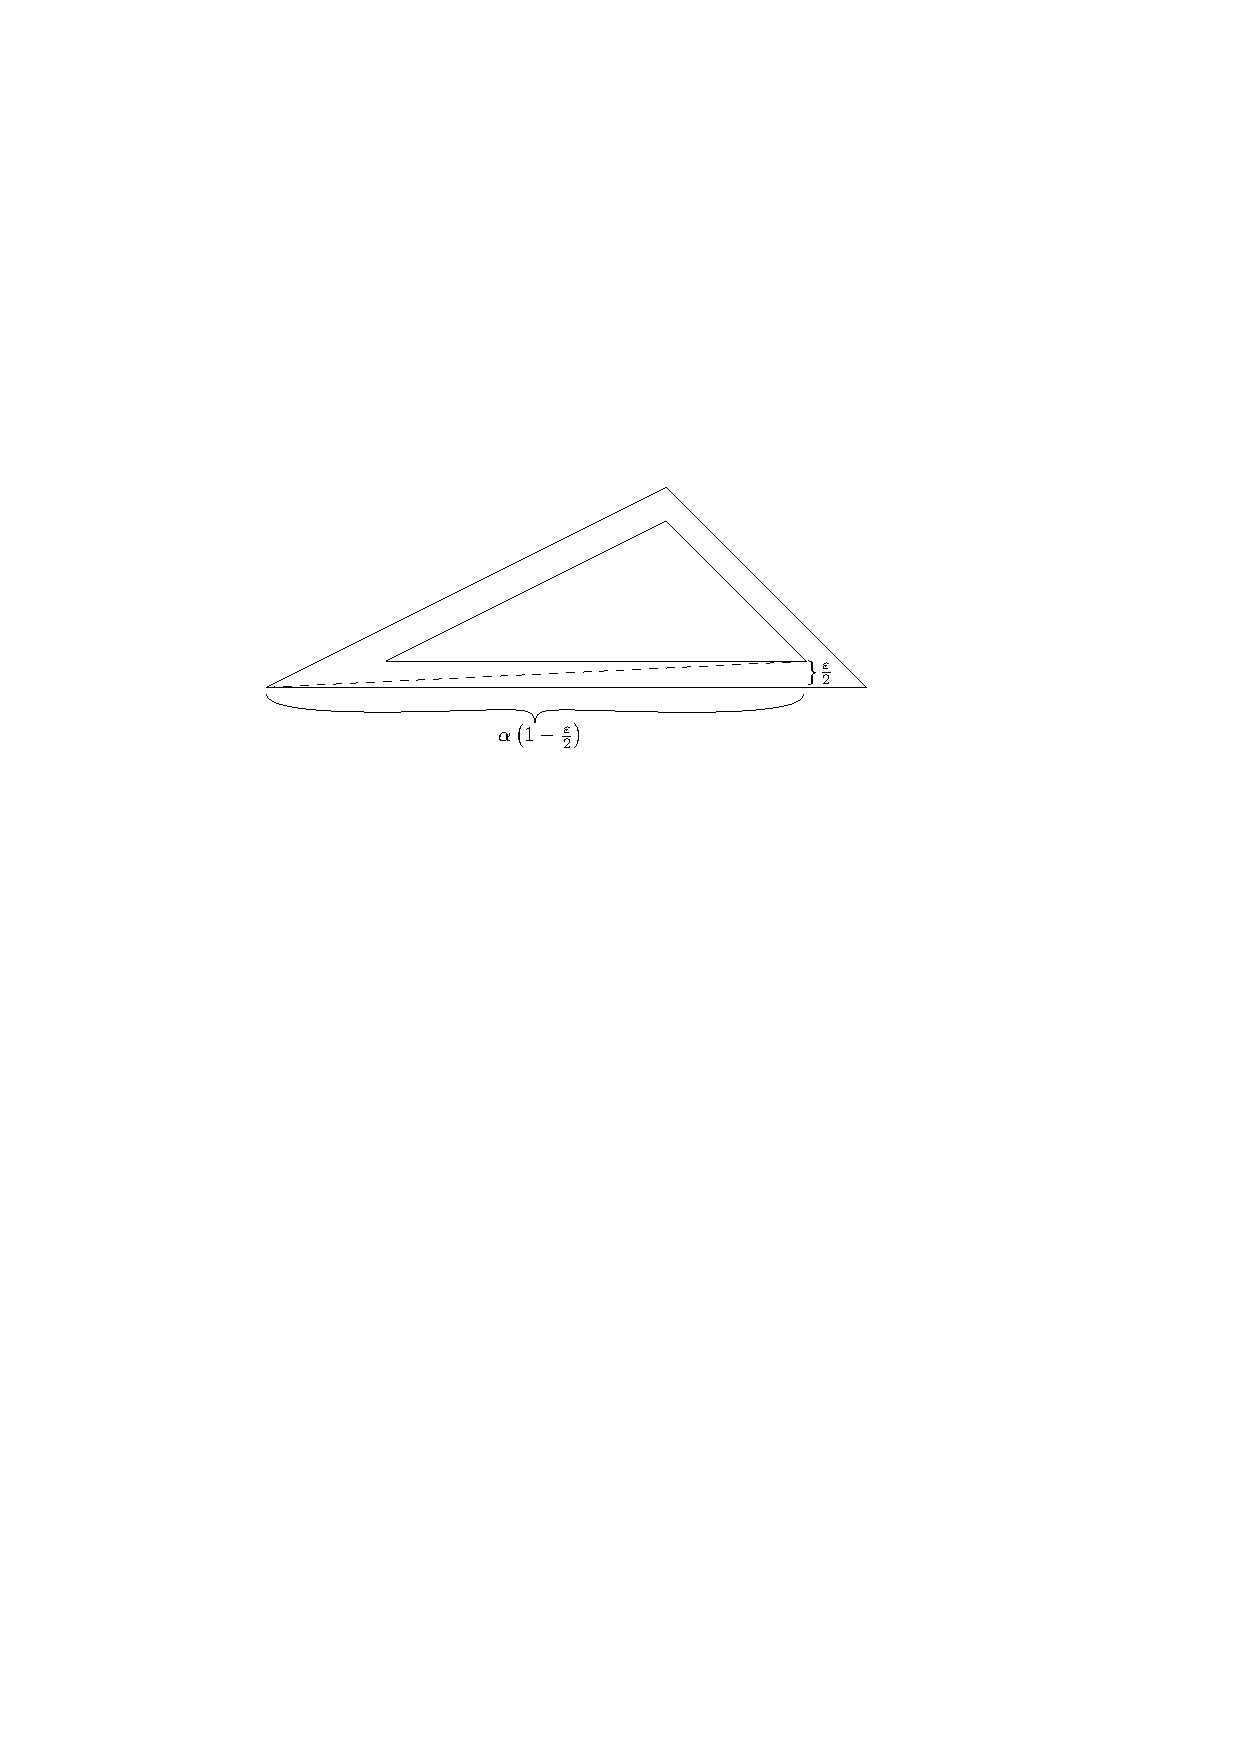
\includegraphics[width=0.6\linewidth]{figs/triangle_shadow}
    \figlab{triangle_with_shadow}
\end{figure}


<<<<<<< HEAD
=======
\subsection{Fat convex regions}

Let $C$ be a convex shape, let $d_+$ be the smallest disk containing $C$, and $d_-$ be the largest disk contained in $C$. We say that $C$ is $\alpha$-fat if the ratio $\frac{radius(d_+)}{radius(d_-)}$ is at most $\alpha$. Let $\LL$ be the set of all $\alpha$-fat convex shapes. In the following, we construct $(\LL, \eps)$-local $t$-spanners for $t>1$. 

We start by proving a structural lemma which will be later used in the correctness proof.

\begin{claim}
	Let $C$ be an $\alpha$-fat convex shape, and let $C_{1-\eps}$ be the $\epsilon$ core of $C$. The shortest segment $\overline{pq}$ such that $p,q\in\partial C$ and $\overline{pq}\cap C_{1-\eps}\neq \emptyset$ is of length at least %TODO.
\end{claim}

\begin{proof}
	Let $d_-$ and $d_+$ be two disks, such that $d_-\subseteq C\subseteq d_+$, and $\frac{radius(d_+)}{radius(d_-)}=\alpha$, and let $\overline{pq}$ be the a shortest segment. We assume $\overline{pq} \cap C_{1-\eps}$ is a single point $s$.
\end{proof}


>>>>>>> 1eb5c890e1265a08cfd6d0936ebc605ac6255af5
\bibliographystyle{alpha} 
%\bibliography{shortcuts,geometry}
\bibliography{ft_spanner}

\end{document}
